\documentclass{atistandalonetask}
\usepackage{atistandard}
\begin{document}
  \begin{atiTask}[
    title = \textsc{Gauß}sche Integrale
  ]
    \begin{atiSubtasks}
    	\item Berechnen Sie das Integral
    	\[
    	I=\integral{0}{\infty}{e^{-x^2}}{x}
    	\]
    	indem Sie zunächst $J=\left(\integral{-\infty}{\infty}{e^{-x^2}}{x}\right)^2$ betrachten und dieses Integral in Polarkoordinaten berechnen und anschließend $I$ aus $J$ berechnen.
    	\item Berechnen Sie (mit Hilfe von (a)) das Integral
    	\[
    	K=\integral{-\infty}{\infty}{e^{-ax^2+bx}}{x},\quad a>0.
    	\]
    \end{atiSubtasks}	
  \end{atiTask}
  \begin{atiSolution}
  Fehler in Musterlösung noch korrigieren->vgl. Bilddatei
	 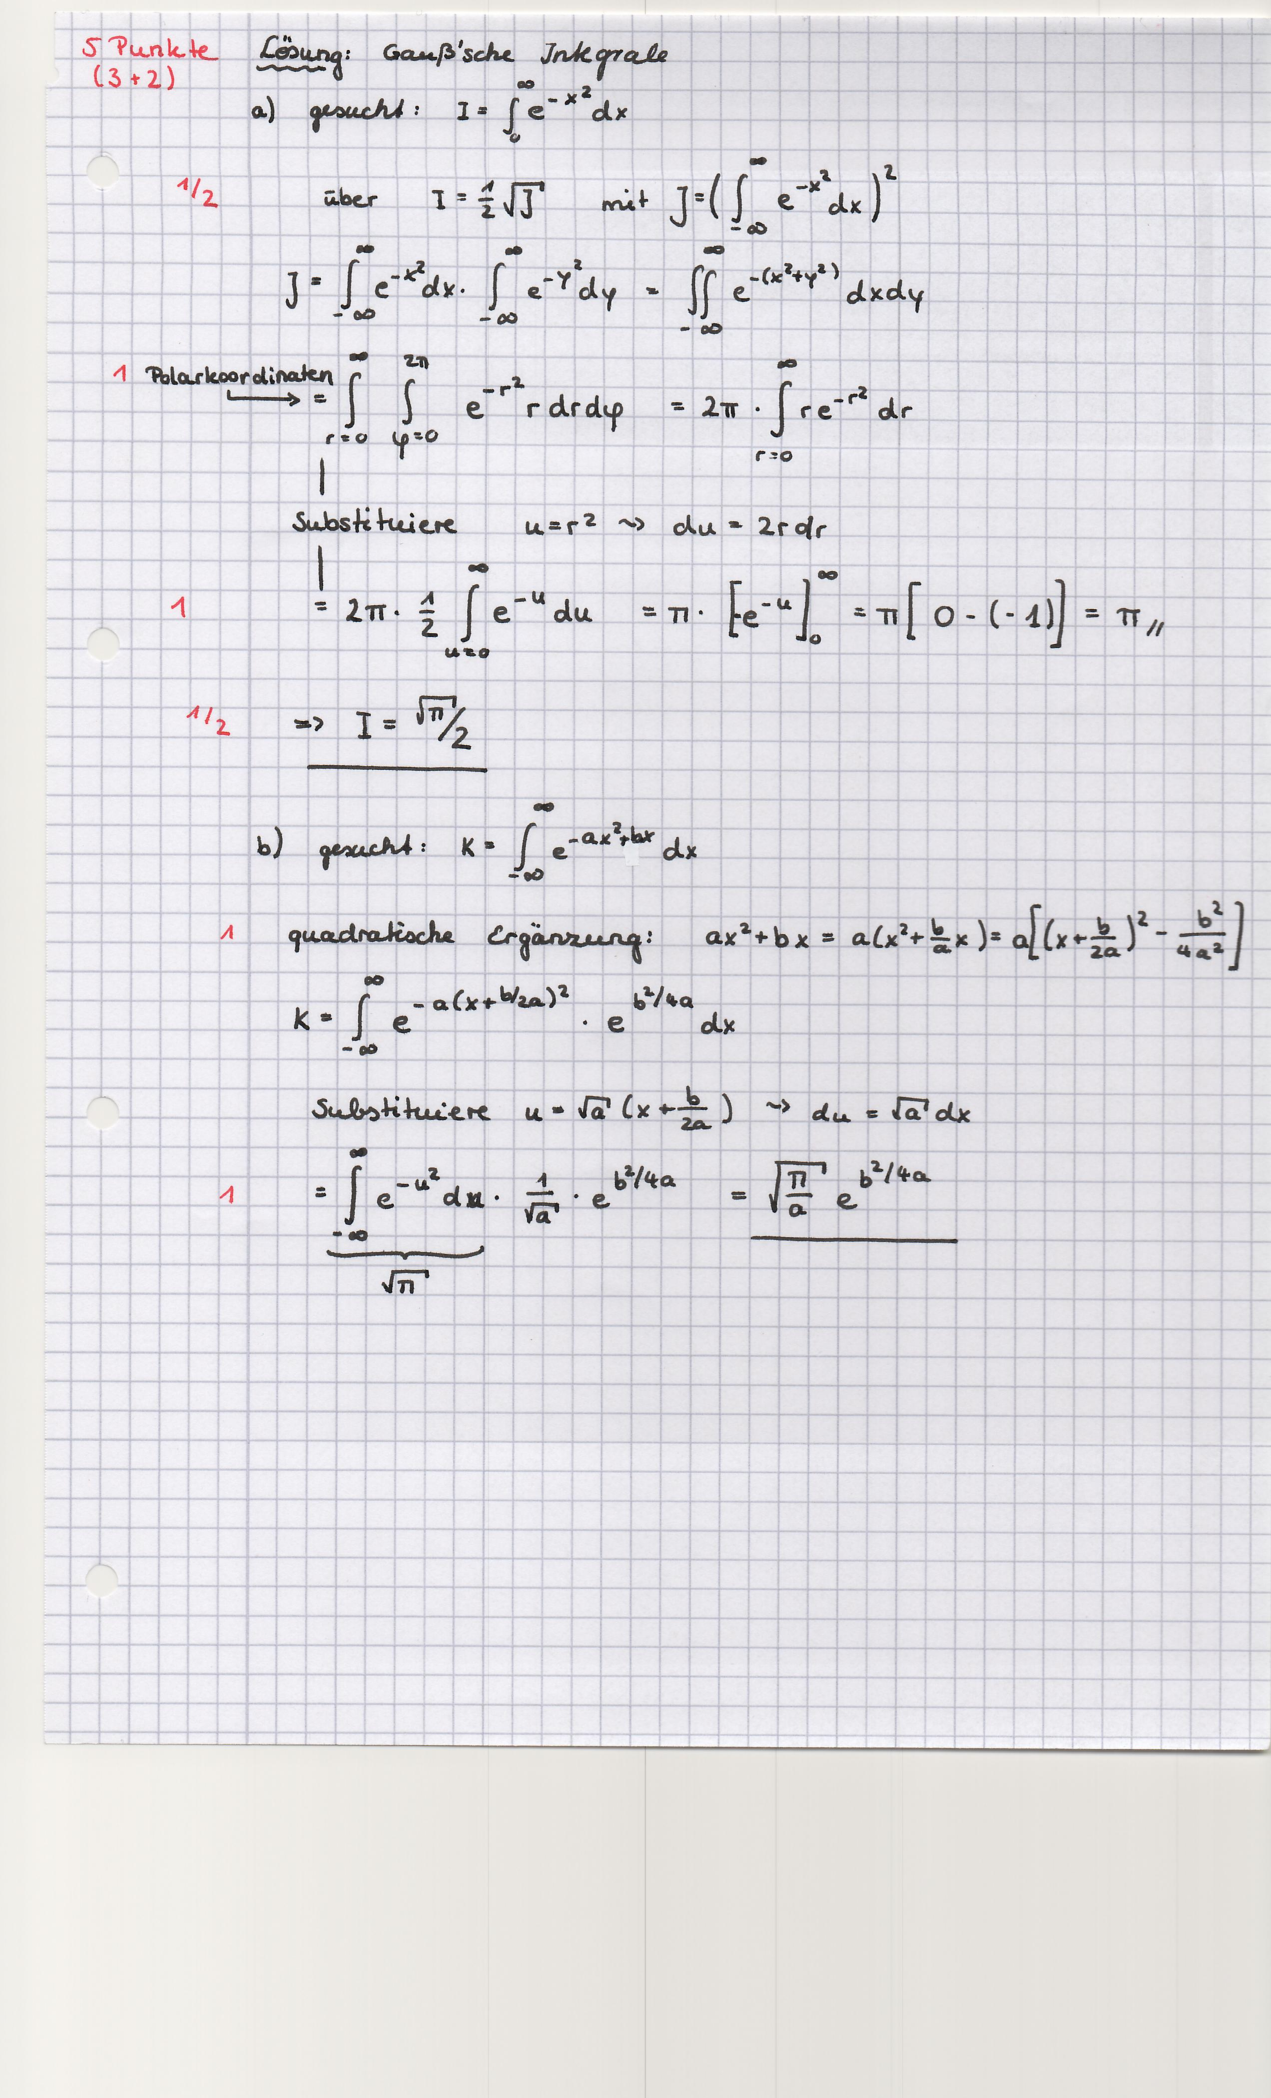
\includepdf[pages=-]{solution-delta_i.pdf}
  \end{atiSolution}
\end{document}